\documentclass{standalone}
\usepackage{tikz}

\begin{document}
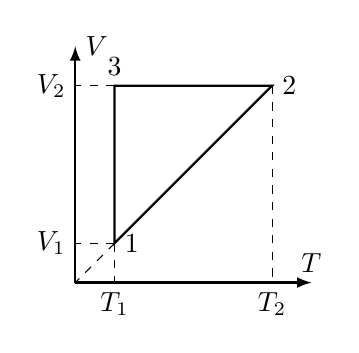
\begin{tikzpicture}
	\draw[thick, arrows={-latex}] (0,0) -- (3,0) node[above] {$T$};
	\draw[thick, arrows={-latex}] (0,0) -- (0,3) node[right] {$V$};
	\draw [thick] (0.5,2.5) node [above] {3} -- (2.5,2.5) node [right] {2} -- (0.5, 0.5) node [right] {1} -- cycle;
	\draw [dashed] (2.5, 2.5) -- (2.5, 0) node [below] {$T_2$};
	\draw [dashed] (0.5, 0.5) -- (0.5, 0) node [below] {$T_1$};
	\draw [dashed] (0.5, 2.5) -- (0,2.5) node [left] {$V_2$};
	\draw [dashed] (0.5, 0.5) -- (0, 0.5) node [left] {$V_1$};
	\draw [dashed] (0.5, 0.5) -- (0, 0);
\end{tikzpicture}
\end{document}